% enable this to activate the version for PRINT
% disable this to make the pdf symmetric and without white pages
% => asymmetric alternating left/right margins
% \newcommand*{\printversion}{}%

%% | ---------------- document meta information --------------- |

\newcommand{\Author}{Yevhenii Kubov}
\newcommand{\Department}{Department of Cybernetics}
\newcommand{\Supervisor}{Ing. Matouš Vrba}
\newcommand{\SupervisorSpecialist}{Ing. My Specialist, Ph.D.}
\newcommand{\Programme}{Cybernetics and Robotics}
%\newcommand{\Field}{TODO}
\newcommand{\Title}{Implementation of a neural network \\[0.5em]for autonomous trail following}
\newcommand{\Keywords}{Unmanned Aerial Vehicles, Robotic Perception, Deep Learning, Convolutional Neural Networks}
\newcommand{\KlicovaSlova}{Bezpilotní Prostředky, Robotické Vnímání, Hluboké Učení, Konvoluční Neuronové Sítě}
\newcommand{\Year}{2022}
\newcommand{\Month}{May}
\newcommand{\Date}{\Month~\Year}
\newcommand{\Location}{Prague}

%% | ---------------------- configuration --------------------- |

% most of the configuration stuff happens here
\input{src/document_setup.tex}

%% | ---------------------- the contents ---------------------- |

\begin{document}

\pagenumbering{roman}

%% --------------------------------------------------------------
%% |                         Title page                         |
%% --------------------------------------------------------------

\input{src/title}

% set up the page style for the "intro" pages
\pagestyle{plain}



%% --------------------------------------------------------------
%% |                         Assignment                         |
%% --------------------------------------------------------------

\conditionalClearPage

\includepdf{src/assignment.pdf}

%% --------------------------------------------------------------
%% |                       Acknowledgments                      |
%% --------------------------------------------------------------

\conditionalClearPage

%!TEX root = ../main.tex

\section*{Acknowledgments}

Firstly, I would like to express my gratitude to my supervisor Ing. Matouš Vrba for his great support and providing all the necessary information during writing this thesis. I'm grateful to the MRS team for guiding me during the experiments.

I would also like to thank my parents, who made it possible for me to study at CTU in Prague and for their support. 

Finally, I would like to express my respect and deep gratitude to my friends, relatives and other people who now, no matter what, defend their home and democracy in Ukraine.



\vspace{2.5cm}



%% --------------------------------------------------------------
%% |                         Statement                          |
%% --------------------------------------------------------------


\conditionalClearPage
\vspace{15cm}
%!TEX root = ../main.tex

~\vfill{}

\section*{Author statement for undergraduate thesis}
\vskip 0.5em
I declare that the presented work was developed independently and that I have listed all sources of information used within it in accordance with the methodical instructions for observing the ethical principles in the preparation of university theses.

Prague, date ................. \hspace{5cm}......................

\section*{Prohlášení autora práce}
\vskip 0.5em
Prohlašuji, že jsem předloženou práci vypracoval samostatně a že jsem uvedl veškeré použité informační zdroje v souladu s Metodickým pokynem o dodržování etických principů při přípravě vysokoškolských závěrečných prací.

V Praze dne ................. \hspace{5cm}......................






\vspace{2.5cm}





%% --------------------------------------------------------------
%% |                          Abstracts                         |
%% --------------------------------------------------------------

\conditionalClearPage

%!TEX root = ../main.tex

\begin{changemargin}{0.8cm}{0.8cm}

~\vfill{}

\section*{Abstract}
\vskip 0.5em

The problem of trail following using image from monocular camera, attached to an unmanned drone or ground vehicle is tackled in this thesis. A system solving the task of flying through the forest along the man-made dirt trail is presented. It is accomplished by using a classification deep convolutional neural network for determining which direction is the camera pointed, relative to the trail. It was implemented to run in real-time onboard MRS multi-rotor drone. Performance and robustness was tested in simulations, followed by real-world experiments. The implemented system showed good practical results and can be used as a starting point for more complex navigation and surveillance applications.

\vskip 1em

{\bf Keywords} \Keywords

\vskip 2.5cm

\end{changemargin}


\conditionalClearPage

%!TEX root = ../main.tex

\begin{changemargin}{0.8cm}{0.8cm}

~\vfill{}

\section*{Abstrakt}
\vskip 0.5em

\sloppy
Tato práce je zaměřená na problematiku sledování lesní cesty pomocí obrázku z monokulární kamery, připevněné na bezpilotní helikoptéře nebo pozemním vozidle. Je představen systém, řešící úlohu navigace podél stezky v lese. To bylo dosaženo s využitím klasifikační hluboké konvoluční neuronové sítě pro určení směru natočení helikoptéry vzhledem k cestě. Systém byl implementován pro běh v reálném čase na bezpilotní helikoptéře MRS. Výkon a robustnost byla otestována v simulaci a následně během experimentů v reálném světe. Implementovaný systém prokázal dobré praktické výsledky a může být použit pro jako výchozí bod pro komplexnější navigační a průzkumné aplikace.

\vskip 1em

{\bf Klíčová slova} \KlicovaSlova

\vskip 2.5cm

\end{changemargin}


%% --------------------------------------------------------------
%% |                        Abbreviations                       |
%% --------------------------------------------------------------

\conditionalClearPage

\begin{changemargin}{0.8cm}{0.8cm}

~\vfill{}

\section*{Abbreviations}

% this will print only the used abbreviations
%!TEX root = ../main.tex

\begin{acronym}
  \acro{CTU}[CTU]{Czech Technical University}
  \acro{FOV}[FOV]{Field of View}
  \acro{GNSS}[GNSS]{Global Navigation Satellite System}
  \acro{GPS}[GPS]{Global Positioning System}
  \acro{IMU}[IMU]{Inertial Measurement Unit}
  \acro{LiDAR}[LiDAR]{Light Detection and Ranging}
  \acro{MAV}[MAV]{Micro Aerial Vehicle}
  \acro{MRS}[MRS]{Multi-robot Systems Group}
  \acro{ROS}[ROS]{Robot Operating System}
  \acro{UAV}[UAV]{Unmanned Aerial Vehicle}
  \acro{UGV}[UGV]{Unmanned Ground Vehicle}
  \acro{RGB}[RGB]{Red Green Blue additive colour model}
  \acro{USB}[USB]{Universal Serial Bus}
  \acro{IR}[IR]{Infrared}
  \acro{CNN}[CNN]{Convolutional Neural Network}
  \acro{DNN}[DNN]{Deep Neural Network}
  \acro{SAR}[SAR]{Search and Rescue}
  \acro{GPU}[GPU]{Graphics Processing Unit}
\end{acronym}


\vskip 2.5cm

\end{changemargin}

\conditionalClearPage

%% --------------------------------------------------------------
%% |                      Table of contents                     |
%% --------------------------------------------------------------

\tableofcontents

\conditionalClearPage

% set up the full page style with normal page numbering
\pagestyle{full}
\pagenumbering{arabic}


\chapter{Introduction}


\section{Unmanned Aerial Vehicles}
Flying robots, also called \acs{UAV}s have been used since the first half of the 20th century \cite{keane2013brief}. They were still controlled by a human operator, but allowed for dangerous tasks to be performed remotely, like aerial target practices. Originally designed for military purposes, they evolved into a vast industry. Since that time, electronic hardware has become much more compact, power-efficient, cheap and advanced. Also, aircraft designs have strongly evolved after decades of research, battery power improved, and software got more advanced. Nowadays, all these factors allow for a wide usage of compact and relatively inexpensive vehicles in many industries and research. 

\acs{UAV}s can be equipped with different payloads and sensors, depending on their task (\reffig{fig:firefighter}). For example, thermal cameras are used for border control \cite{abushahma2019comparative, pedrozo2017swiss, girard2004border}, detecting animals in wildlife \cite{chretien2015wildlife, lhoest2015many}, or forest fires \cite{yuan2017fire, merino2005cooperative}. \acs{LiDAR}s can be used for 3D mapping of a designated area \cite{lin2019evaluation}, for navigation in an obstructed environment. Digital cameras are utilised for crops analysis \cite{paredes2017multispectral, yue2018comparison}, area mapping \cite{nex2014uav}, surveillance \cite{girard2004border}, monitoring of different constructions or power lines \cite{zhang2017uav}. 


\begin{figure}[!h]
  \centering
  \includegraphics[width=0.6\textwidth]{./fig/photos/firefighter.jpeg}

  \caption{\acs{MRS} \acs{MAV} equipped with firefighting and thermal imaging modules.}
  \label{fig:firefighter}
\end{figure}


\acs{UAV}s are also important for \ac{SAR} missions. Benefits of using them in such operations is that these vehicles are usually portable, have small deployment time and generally require only minimal qualification to operate them, thanks to flight computers with advanced software \cite{erdos2013experimental, goodrich2008supporting}. They can be used instead of human teams, reducing the risk for their life or health in dangerous environments. \acs{UAV}s may be also cheaper than alternatives, especially manned aircraft, and faster than rescue teams or ground vehicles. They are usually not only less expensive, but also provide data logging from all sensors, including \acs{GPS} and associated image data from high resolution cameras. This data can be used even for later review. For \acs{SAR} missions, typically two types of \acs{UAV}s are used: fixed-wing aircraft and multi-rotor helicopters. The first ones provide higher speed, flight time, but are less agile and take longer time to take off and land the vehicle. Multi-rotors have the ability to hover, fly close to the ground, in buildings, caves and other complex terrains. In this thesis, a multi-rotor \acs{MAV} will be used as an airframe. 


\section{Convolutional neural networks}

Neural networks (also called artificial neural networks) are algorithms, whose design was inspired by biological neural networks in human and animal brains. Their structure consists of nodes called neurons, and connections between them. Every connection has its weight. Neurons are grouped into layers, each layer has its unique number of them. Neurons which receive value (stimuli) on input from outside of the network are input neurons. Those which receive values from other neurons, process this data, and output the result to other neurons are hidden neurons. Those which output the result outside the network are called output neurons. The mentioned weights of connections between the neurons can be adjusted through a learning process. During learning, a network learns to identify needed templates in the input and produce a correct decision according to the task. 

Convolutional neural networks have been experiencing tremendous growth during the last 10 years, allowing for many previously unsolved problems to be tackled \cite{li2021survey}. They are used in military, healthcare, aerospace, social media, science and other applications. This approach allowed for faster and more accurate analysis of many diseases even on early stages \cite{zhou2018unet++}, using measurements performed on the patient, which are then fed to a neural network. In aerospace and automotive engineering neural networks are often used as component fault detectors and for improved guidance systems \cite{yaqoob2019autonomous}. In electronics their capabilities help to expose failures when producing the chips, synthesise voice, compress data and solve many other tasks \cite{gomez2016neural, goyal2018deepzip}. In military they help to identify hostile objects or enemies \cite{wu2015typical}. 


There are different types of neural networks. Several examples are presented in this chapter.

\subsection{Segmentation networks}
Among the most popular types are segmentation neural networks. Their goal is to divide an image into multiple segments. In such architecture, each pixel refers to some class or object type. This type is often used for biomedical applications. A good example is the U-Net architecture, frequently used in light microscopy \cite{ronneberger2015u}.

\subsection{Recurrent networks}

This type of networks is used for problems, such as language translation and speech recognition. They are designed to handle sequential data on input (\reffig{fig:recurrent}).

\begin{figure}[!h]
  \centering
  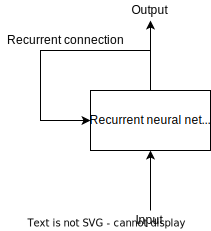
\includegraphics[width=0.5\textwidth]{./fig/photos/recurrent.pdf}

  \caption{Example of a recurrent network architecture.}
  \label{fig:recurrent}
\end{figure}

\subsection{Generative adversarial networks}

GAN networks consist of two neural networks, that contest with each other. Each network's gain is another network's loss. For example, in the problem of generating realistic-looking images, one network called discriminator identifies how much the input image is \enquote{realistic}, while the other (generator) generates this input and adjusts it to \enquote{fool} the discriminator.

\subsection{Classification networks}

One of the most popular are classification neural networks. In such use-case given an input image, a neural network must identify to which class does an image belong. Good example is the Alexnet architecture for classification on 1000 classes subset from the ImageNet dataset \cite{krizhevsky2012imagenet}. Back in 2012, it won the ImageNet large-scale visual recognition challenge. This type of a neural network is used in this thesis. However, more modern and suitable architecture from \cite{giusti2016machine} is employed.

\section{Trail following}

In this thesis, the problem of trail following using image from monocular camera onboard a multi-rotor \acs{MAV} is tackled, including the implementation of a working algorithm, solving the task. Following the man-made forest path is natural for humans, because it is usually the most efficient way to get through this complex terrain. Such policy, in most cases, minimises the travel time and possible injury to a person (\reffig{fig:challenging_path}). The same applies to robots. Human paths are freely passable, unlike random trajectories in a forest, and it is a reason to stay on them.

\begin{figure}[!h]
  \centering
  \includegraphics[width=0.75\textwidth]{./fig/photos/challenging_path.jpg}

  \caption{Random path in a forest is generally challenging to pass.}
  \label{fig:challenging_path}
\end{figure}

Trail following is an important task for autonomous navigation of robots. Suggested use-cases are search and rescue missions, efficient navigation through forests and mapping of the area. Motivation for this task is a situation when there is no opportunity to communicate with and control the vehicle manually or when an autonomous mission is highly preferred. The goal is to allow for a quadcopter or an unmanned ground vehicle (UGV) to navigate through a forest using computer vision techniques. Having the image from the onboard camera, the vehicle should determine in which direction to travel when flying through a forest, to utilise the trail. It must strictly follow the human path.

Algorithms solving related problems like lane-following, lane-departure and lane-assist for cars on public roads, were introduced in 1990's \cite{batavia1999driver} and are commonly used in personal vehicles since the early 2000's \cite{chen2020lane}. But there is a clear distinction between the lane on a road and a forest trail. In the first case, the lane is marked with contrast symbols and lines, making the task solvable by simple segmentation algorithms, based on in-image contrast and colour variance, image saliency \cite{santana2013tracking}. Forest trail images provide smaller amount of distinguishable features (\reffig{fig:features_difference}) and it may be challenging even for humans to determine the direction of travel \cite{giusti2016machine}.

\begin{figure}[H]
  \centering
  \subfloat[Image of a trail from the dataset \cite{giusti2016machine}.] {
    \includegraphics[width=0.45\textwidth]{./fig/photos/trail1.jpg}
    \label{fig:trail_1}
  }
  \subfloat[Image of a road taken by myself.] {
    \includegraphics[width=0.45\textwidth]{./fig/photos/road.PNG}
    \label{fig:road_1}
  }
  \caption{Difference between a forest trail on \reffig{fig:trail_1} and a road on \reffig{fig:road_1}.}
  \label{fig:features_difference}
\end{figure}

One of the first effectively solved by neural networks but still topical problems is classification. Neural networks are able to learn and then identify features corresponding to pre-defined classes and combinations of those features \cite{krizhevsky2012imagenet}. This makes it possible to effectively classify which class an image belongs to. 

Treating the trail following task as a classification problem is a different approach that tackles it. For this approach, classes like "Left", "Right" and "Straight" can be introduced \cite{giusti2016machine} (\reffig{fig:classes}). It allows to estimate the current direction of a vehicle, given the probabilities of these classes and to plan the trajectory of the \acs{MAV} accordingly. 


\begin{figure}[!h]
  \begin{minipage}{.5\linewidth}
  \centering
  \subfloat[Class "left".] {
    \includegraphics[width=0.95\textwidth]{./fig/photos/class_l.jpg}
    \label{fig:class_l}
  }
  \end{minipage}
  \begin{minipage}{.5\linewidth}
  \centering	
  

  \subfloat[Class "right".] {
    \includegraphics[width=0.95\textwidth]{./fig/photos/class_r.jpg}
    \label{fig:class_s}
  }
  \end{minipage}\par\medskip
  \centering
  \subfloat[Class "straight".] {
    \includegraphics[width=0.5\textwidth]{./fig/photos/class_s.jpg}
    \label{fig:class_r}
  }
  \caption{Example images of different classes.}
  \label{fig:classes}
\end{figure}

This thesis focuses on implementation of the trail-following algorithm using a classification convolutional neural network. The implementation should run online in the Gazebo simulation environment as well as onboard an \acs{MAV} in a real-world deployment. Therefore, delay of the algorithm must be sufficiently small. The task is to design an algorithm that autonomously provides an \acs{MAV} with a relatively safe direction and speed of movement. The \acs{MAV} is equipped with a PX4 flight computer, an Intel NUC companion computer, and an Intel RealSense camera. The environment may contain obstacles, but it is assumed that the trail is obstacle-free. 

Implemented neural network can be used as an entry point for a more sophisticated surveillance and navigation algorithms. For more complex environments a possible enhancement is to use it alongside with an obstacle avoidance algorithms and lateral correction \cite{back2020autonomous, maciel2018extending, smolyanskiy2017toward}.















\chapter{Methodology}

In this thesis, an architecture suggested by \citeauthor{giusti2016machine} \cite{giusti2016machine} will be used. It consists of 4 convolutional layers, each followed by a hyperbolic tangent activation function and max-pooling layer, and then a fully connected layer with 200 hidden neurons. Network processes images from a camera, attached to a vehicle. Input layer is formed by $3\times 101\times101$ neurons. Therefore, the input \acs{RGB} rectangular image must be anisotropically resized to a size $101\times101$ pixels (square) to be fed directly to the network. After going through all the hidden layers and the softmax output layer, it produces 3 probabilities of each class, which sum to 1. Based on these probabilities, it is possible to determine at which direction is the camera most probably pointed. Given the fact that in the dataset the cameras for "left" and "right" classes were pointed $30 \degree$ from the centre, interpolation is also possible based on these probabilities.  


\section{Convolutional Neural Network}
\subsection{Convolutions}

Convolution is a fundamental mathematical operation used in a wide range of image processing techniques. In the context of Convolutional Neural Networks, convolution of an input matrix $I$ with a so called "kernel" matrix $K$ is applied to obtain an output matrix $O$. The kernel is typically smaller and is applied to submatrices of $I$ to extract features corresponding to $K$ in different regions of $I$. The convolutional layer of a \acs{CNN} typically also contains a bias term $w_0$. The kernel matrix $K$ and the bias $w_0$ are parameters that are learned during the training phase using the backpropagation algorithm, described in section \ref{backprop}. Let us define
\begin{equation}
	I = \begin{bmatrix}
    x_{11}       & x_{12} & x_{13} & \dots & x_{1n} \\
    x_{21}       & x_{22} & x_{23} & \dots & x_{2n} \\
    \hdotsfor{5} \\
    x_{r1}       & x_{r2} & x_{r3} & \dots & x_{rn}
\end{bmatrix}\,,
\label{Input data}
\end{equation}

\begin{equation}
	K = \begin{bmatrix}
    w_{11}       & w_{12} & w_{13} \\
    w_{21}       & w_{22} & w_{23} \\
    w_{31}       & w_{32} & w_{33} 
	\end{bmatrix}\,.
\label{Kernel}
\end{equation}

Convolution is performed by "stamping" a kernel onto the input data, starting from the upper left angle and thus creating a linear combination of input array members and kernel weights. The result of the first application of the convolution kernel will be

\begin{equation}
\begin{aligned}
	O(1, 1) = x_{11}\cdot w_{11} + x_{12}\cdot w_{12} + x_{13}\cdot w_{13} +\\
	x_{21}\cdot w_{21} + x_{22}\cdot w_{22} + x_{23}\cdot w_{23} + \\
	x_{31}\cdot w_{31} + x_{32}\cdot w_{32} + x_{33}\cdot w_{33} + w_0\,.
\end{aligned}
\end{equation}

And the equation for the convolutional kernel stamp starting on i-th row and j-th column of the input image (where the convolution is defined) is

\begin{equation}
	O(i, j) = w_0 + \sum\limits_{k=1}^m \sum\limits_{l=1}^n I_{i+k-1, j+l-1}\cdot K_{k, l} \,,
\end{equation}
where kernel has $m$ rows and $n$ columns, $i$ runs from 1 to $M-m+1$, $j$ runs from 1 to $N-n+1$. To produce the output array, the filter must slide through the whole input image.


\subsection{Hyperbolic tangent}

For a neural network to not act as a linear classifier, a nonlinearity should be introduced in its hidden layers \cite{sharma2017activation}. It allows the network to solve more complex tasks and increase its performance. It is also a nature-inspired approach. Nonlinearity is introduced using nonlinear activation layers, added after each convolutional layer. The most popular activation functions are Rectified Linear Unit (ReLU), Leaky ReLU, Sigmoid and Hyperbolic Tangent. The last one is used in this thesis. Hyperbolic Tangent has a very similar shape to the Sigmoid and also maps the output only to the range of [-1, 1] (\reffig{fig:htangent}). It is calculated using the following equation:
\begin{equation}
	\textrm{tanh}(x) = \frac{e^x-e^{-x}}{e^x+e^{-x}}\,,
\end{equation}
where $x$ is the real input value obtained after the convolution stamp.

\begin{figure}[!h]
  \centering
  \includegraphics[width=0.6\textwidth]{./fig/photos/hyperbolic_tangent.png}

  \caption{A Hyperbolic Tangent function.}
  Author: Geek3, CC BY-SA 3.0, https://commons.wikimedia.org/w/index.php?curid=4198479
  \label{fig:htangent}
\end{figure}


\subsection{Max-pooling}

Max-pooling is an operation applied to some part of the input data array taking only the maximum value of this area. It is typically used in the form of a rectangular filter, which slides through the whole image. It produces only one output value from each filter-sized input area. Thus, it can be used for downsampling the image, taking only the most significant values to the output. In this way, the learning process of the neural network is sped up because the amount of learnable weights is decreased. Also, better resistance to distortions and affine transformations is obtained \cite{yu2014mixed}.

\subsection{Softmax}

The softmax function is widely used in neural network architectures as the last layer. It has the same amount of outputs as inputs. The softmax function may have any real values on input, including positive, negative, zero, but its output values are always in the range $[0, 1]$ and they always sum to 1. These properties allow the output to be interpreted as a probability distribution of the corresponding classes. This layer normalises the output, which is from $\textrm{R}^n$ to a probability distribution.

The softmax function is defined as:

\begin{equation}
	\sigma(\vec z)_i = \frac{e^{z_i}}{\sum\limits_{j=1}^n e^{z_j}}\,,
\end{equation}
where $z_i$ are elements of the real input vector, $\sigma(\vec z)$ is the output vector, $n$ is the number of elements.




\section{Backward propagation of error}
\label{backprop}

Backward propagation is a way to calculate the gradient $\frac{\partial J}{\partial \textbf{w}}$ of the loss function $J$ with respect to the vector of weights $\textbf{w}$\,. The calculated gradient has the same length as the weights vector. It represents how much each weight affects and contributes to the value of the loss function. This knowledge is used to change the weights in a way that minimises the loss. 

The first part of backpropagation is a forward pass. Given the input data and the weights, output of the neural network is calculated and compared with ground truth through the loss function. Then, a backward pass starts. Partial derivatives are calculated sequentially through each layer starting from the last one and after multiplication give the total gradient $\frac{\partial J}{\partial \textbf{w}}$\,.

The architecture used in this thesis consists of convolutional layers, max-pooling layers, a hyperbolic tangent activation function and fully connected layers (\reffig{fig:architecture}). Max-pooling chooses one input with the maximum value and feeds it directly to the output, other inputs are ignored. It doesn't have learnable parameters affecting the gradient. During backpropagation, the gradient is only propagated to the maximal input, the remaining non-maximal inputs have a zero gradient. The derivative of the hyperbolic tangent is $\frac{d\textrm{tanh}(x)}{dx} = 1-\textrm{tanh}(x)^2$. In the convolutional layer, back propagation is the convolution of the input feature map with the upstream gradient (\reffig{fig:conv_bp}). In the figure, $\gamma(y)$ is any function, for example the activation function. In this case, backpropagation through the convolution will be:
\begin{equation}
\begin{aligned}
	\frac{\partial \gamma}{\partial w_{11}} = \frac{\partial\gamma}{\partial y_{11}} x_{11} + \frac{\partial\gamma}{\partial y_{12}} x_{12} + \frac{\partial\gamma}{\partial y_{21}} x_{21} + \frac{\partial\gamma}{\partial y_{22}} x_{22}\,, \\
	\frac{\partial \gamma}{\partial w_{12}} = \frac{\partial\gamma}{\partial y_{11}} x_{12} + \frac{\partial\gamma}{\partial y_{12}} x_{13} + \frac{\partial\gamma}{\partial y_{21}} x_{22} + \frac{\partial\gamma}{\partial y_{22}} x_{23}\,, \\
	\frac{\partial \gamma}{\partial w_{21}} = \frac{\partial\gamma}{\partial y_{11}} x_{21} + \frac{\partial\gamma}{\partial y_{12}} x_{22} + \frac{\partial\gamma}{\partial y_{21}} x_{31} + \frac{\partial\gamma}{\partial y_{22}} x_{32}\,, \\
	\frac{\partial \gamma}{\partial w_{22}} = \frac{\partial\gamma}{\partial y_{11}} x_{22} + \frac{\partial\gamma}{\partial y_{12}} x_{23} + \frac{\partial\gamma}{\partial y_{21}} x_{32} + \frac{\partial\gamma}{\partial y_{22}} x_{33}\,.
\end{aligned}
\end{equation}

\begin{figure}[H]
  \centering
  
  \documentclass{standalone}
\usepackage{pgfplots}
\usepackage{bm}
\usepackage{siunitx}
\pgfplotsset{compat=1.12}
\usetikzlibrary{arrows, decorations.pathmorphing, backgrounds, positioning,fit,petri}
\usetikzlibrary{calc}

\newcommand{\xdistl}{6cm}
\newcommand{\xdistr}{4cm}

\begin{document}

\begin{tikzpicture}
  \fontsize{11}{11}
  {
    \node[black, draw, thick, rounded corners] (f1) at (0, 0) {Input image 101x101x3};
    \node[black, draw, thick, rounded corners] (f2) [below=of f1] {Feature map 98x98x32};
    \node[black, draw, thick, rounded corners] (f3) [below=of f2] {Feature map 49x49x32};
    \node[black, draw, thick, rounded corners] (f4) [below=of f3] {Feature map 46x46x32};
    \node[black, draw, thick, rounded corners] (f5) [below=of f4] {Feature map 23x23x32};
    \node[black, draw, thick, rounded corners] (f6) [below=of f5] {Feature map 20x20x32};
    \node[black, draw, thick, rounded corners] (f7) [below=of f6] {Feature map 10x10x32};
    \node[black, draw, thick, rounded corners] (f8) [below=of f7] {Feature map 8x8x32};
    \node[black, draw, thick, rounded corners] (f9) [below=of f8] {Feature map 4x4x32};
    \node[black, draw, thick, rounded corners] (f10) [below=of f9] {200 hidden neurons};
    \node[black, draw, thick, rounded corners] (f11) [below=of f10] {3 neurons};



    \draw[->, line width=2pt] (f1.south) -| (f2.north);
    \draw[->, line width=2pt] (f2.south) -| (f3.north);
    \draw[->, line width=2pt] (f3.south) -| (f4.north);
    \draw[->, line width=2pt] (f4.south) -| (f5.north);
    \draw[->, line width=2pt] (f5.south) -| (f6.north);
    \draw[->, line width=2pt] (f6.south) -| (f7.north);
    \draw[->, line width=2pt] (f7.south) -| (f8.north);
    \draw[->, line width=2pt] (f8.south) -| (f9.north);
    \draw[->, line width=2pt] (f9.south) -| (f10.north);
    \draw[->, line width=2pt] (f10.south) -| (f11.north);



    \node[black, draw, opacity=0, text opacity=1, anchor=west] (l1) at ( $ (f1)!0.5!(f2) + (2, 0)$ ) {Convolution, 4x4 kernel, 1 stride, no padding, tanh activation};
    \node[black, draw, opacity=0, text opacity=1, anchor=west] (l2) at ( $ (f2)!0.5!(f3) + (2, 0)$ ) {Max-pooling, 2x2 kernel, 2 stride, no padding};
    \node[black, draw, opacity=0, text opacity=1, anchor=west] (l3) at ( $ (f3)!0.5!(f4) + (2, 0)$ ) {Convolution, 4x4 kernel, 1 stride, no padding, tanh activation};
    \node[black, draw, opacity=0, text opacity=1, anchor=west] (l4) at ( $ (f4)!0.5!(f5) + (2, 0)$ ) {Max-pooling, 2x2 kernel, 2 stride, no padding};
    \node[black, draw, opacity=0, text opacity=1, anchor=west] (l5) at ( $ (f5)!0.5!(f6) + (2, 0)$ ) {Convolution, 4x4 kernel, 1 stride, no padding, tanh activation};
    \node[black, draw, opacity=0, text opacity=1, anchor=west] (l6) at ( $ (f6)!0.5!(f7) + (2, 0)$ ) {Max-pooling, 2x2 kernel, 2 stride, no padding};
    \node[black, draw, opacity=0, text opacity=1, anchor=west] (l7) at ( $ (f7)!0.5!(f8) + (2, 0)$ ) {Convolution, 4x4 kernel, 1 stride, 1 padding, tanh activation};
    \node[black, draw, opacity=0, text opacity=1, anchor=west] (l8) at ( $ (f8)!0.5!(f9) + (2, 0)$ ) {Max-pooling, 2x2 kernel, 2 stride, no padding};
    \node[black, draw, opacity=0, text opacity=1, anchor=west] (l9) at ( $ (f9)!0.5!(f10) + (2, 0)$ ) {Fully connected layer};
    \node[black, draw, opacity=0, text opacity=1, anchor=west] (l10) at ( $ (f10)!0.5!(f11) + (2, 0)$ ) {Output};



    \node[black, draw, opacity=0, text opacity=1, anchor=west] (ll1) at ( $ (f1)!0.5!(f2) - (3, 0)$ ) {Layer 1};
    \node[black, draw, opacity=0, text opacity=1, anchor=west] (ll2) at ( $ (f2)!0.5!(f3) - (3, 0)$ ) {Layer 2};
    \node[black, draw, opacity=0, text opacity=1, anchor=west] (ll3) at ( $ (f3)!0.5!(f4) - (3, 0)$ ) {Layer 3};
    \node[black, draw, opacity=0, text opacity=1, anchor=west] (ll4) at ( $ (f4)!0.5!(f5) - (3, 0)$ ) {Layer 4};
    \node[black, draw, opacity=0, text opacity=1, anchor=west] (ll5) at ( $ (f5)!0.5!(f6) - (3, 0)$ ) {Layer 5};
    \node[black, draw, opacity=0, text opacity=1, anchor=west] (ll6) at ( $ (f6)!0.5!(f7) - (3, 0)$ ) {Layer 6};
    \node[black, draw, opacity=0, text opacity=1, anchor=west] (ll7) at ( $ (f7)!0.5!(f8) - (3, 0)$ ) {Layer 7};
    \node[black, draw, opacity=0, text opacity=1, anchor=west] (ll8) at ( $ (f8)!0.5!(f9) - (3, 0)$ ) {Layer 8};
    \node[black, draw, opacity=0, text opacity=1, anchor=west] (ll9) at ( $ (f9)!0.5!(f10) - (3, 0)$ ) {Layer 9};
    \node[black, draw, opacity=0, text opacity=1, anchor=west] (ll10) at ( $ (f10)!0.5!(f11) - (3, 0)$ ) {Layer 10};

}
\end{tikzpicture}

\end{document} 

  
  \caption{The employed neural network architecture \cite{giusti2016machine}.}
  \label{fig:architecture}
\end{figure}


% Input ^ adds 600 words, idk why


\begin{figure}[!h]

  \centering
  \includegraphics[width=0.75\textwidth]{./fig/photos/Conv_BP.pdf}
  \caption{Upstream gradient in convolutional layer.}
  \label{fig:conv_bp}
\end{figure}



\section{Loss function}

To train the neural network, it is necessary to define a suitable loss function. It estimates the penalty of the difference between a ground truth and a prediction of the neural network. The loss function outputs one real value based on this data. Then, using the back propagation, the penalty gets minimised. In this thesis, I use a cross-entropy loss criterion. Its equation is

\begin{equation}
	Loss = -\sum\limits_{x=0}^n p(x)\cdot \textrm{log} \,q(x) \,,
\end{equation}
where $n$ is the number of classes, $p(x)$ is the desired probability of the class (ground truth), $q(x)$ is the prediction from the neural network.




\chapter{Implementation}

\section{System hardware}

Main hardware elements are shown on the \reffig{fig:system}. 

\begin{figure}[!h]
  \centering
  \includegraphics[width=0.7\textwidth]{./fig/photos/system.pdf}
  \caption{Scheme of the employed system.}
  \label{fig:system}
\end{figure}

\subsection{Pixhawk flight controller}

Pixhawk is a low-cost advanced flight computer with open-source hardware. There are different variations of form factors, featuring different amount of input/output ports. Pixhawk is very flexible in terms of attachable peripherals, stable and well-tested. Most essential sensors like accelerometers, gyro, digital compass (magnetometer) and barometer are already part of the main board. \acs{MRS} vehicles have these boards flashed with open-source PX4 autopilot software. Features like advanced regulators, estimators, interface for controlling the \acs{MAV} and others are already implemented in this software, usually only minor tweaking is needed. Thus an abstraction from the \acs{MAV} hardware is created, allowing the vehicle to be controlled using high-level commands.


\subsection{Intel NUC companion computer}

NUC is a compact high-performance computer, capable of running demanding AI and machine learning software. It is possible to install the whole \acs{MRS} system on it including \acs{ROS} software to command trajectories, speed and other parameters to a flight controller and act as a main high-level computational unit. \acs{ROS} runs inside the Ubuntu operating system on this computer, so other software can be used simultaneously. Different peripherals can be connected to the computer via \acs{USB}. For this thesis, a RealSense camera is connected, from which my algorithm (written in the Python programming language) receives images for processing.

\subsection{Intel RealSense D435 camera}

The D435 is a powerful camera capable of taking normal \acs{RGB} pictures as well as depth images. It has a wide \acs{FOV}, which is perfect for robotic applications. Also, its stereo imagers feature global shutter, which is important in low-light conditions or during fast movements. The camera consists of 4 modules: a right imager, an \acs{IR} projector, a left imager and an \acs{RGB} module. However, for this thesis only the \acs{RGB} module will be used. Its sensor has a resolution of 2\,MP and produces $1920\times1080$ images at the frame rate of 30 frames per second.


\section{Dataset}

For this task was chosen a dataset from the authors of the \acs{CNN} architecture \cite{giusti2016machine}, but any similar dataset can be used. Requirement is that every image must be labeled to one of the three classes. The used dataset was acquired by a hiker, wearing three head-mounted cameras: one pointing straight ahead, one pointing 30 degrees left, one pointing 30 degrees right. In the code, there will be classes LEFT (for the camera pointed 30 degrees left), STRAIGHT (forward camera), and RIGHT (for the camera pointed 30 degrees right). Dataset is divided in such a way that approximately 75\% of it is used for training, and 25\% for validation. So, the neural network estimates the current direction relative to the trail, and based on this knowledge, further decision can be made.

Dataset was provided by the authors only as a set of photos. For the preparation of these photos into usable form, I implemented a dedicated program in the Python programming language. The program iterates through all images from the dataset and performs transformations so that the images correspond to the required format. In this case, they are resized to 101 by 101 pixels. Images are saved to the python dictionary under fields ‘data’ and ‘label’.

\section{Neural network code}

The implementation of the neural network was not provided by the authors of the architecture. Therefore, it was created by me. I have chosen the Python programming language for this task. It has a lot of available powerful frameworks, especially for machine learning and neural networks, which are internally implemented in faster low-level languages like C++. The PyTorch framework was chosen. It is a powerful open-source machine learning framework for the Python. The PyTorch is capable of running on a \acs{GPU} to accelerate tensor computing, however, CUDA-capable Nvidia \acs{GPU} must be used. In this thesis, it was used on the drone PC without the hardware acceleration.

The neural network is trained for 90 epochs, with a batch size of 512, but even larger size could be considered if the GPU has enough memory. The Adam optimizer is used, with an initial learning rate of 0.005. A scheduler is set, for reducing the learning rate by 5\% after each epoch. The criterion for training is the cross-entropy loss. 

During the training process, the validation accuracy got to the value of 90 percent (\reffig{fig:accuracy}). The process was stopped on 90 epochs because the validation loss has converged (\reffig{fig:loss}). Further training will cause overfitting and worse performance.

\subsection{Training algorithm}

After the initialization of the neural network model, optimizer, scheduler, and criterion, the program enters a 90-epoch loop. Then starts the training part where the forward pass and the back-propagation are calculated, optimizer step is done. After that, validation part begins and the scheduler step is performed. In the end, after a sufficient amount of iterations the weights of the neural network are saved for further usage.

\begin{figure}[!h]
  \centering
  \includegraphics[width=0.7\textwidth]{./fig/photos/accuracy1.eps}
  \caption{Accuracy during the training process.}
  \label{fig:accuracy}
\end{figure}

\begin{figure}[!h]

  \centering
  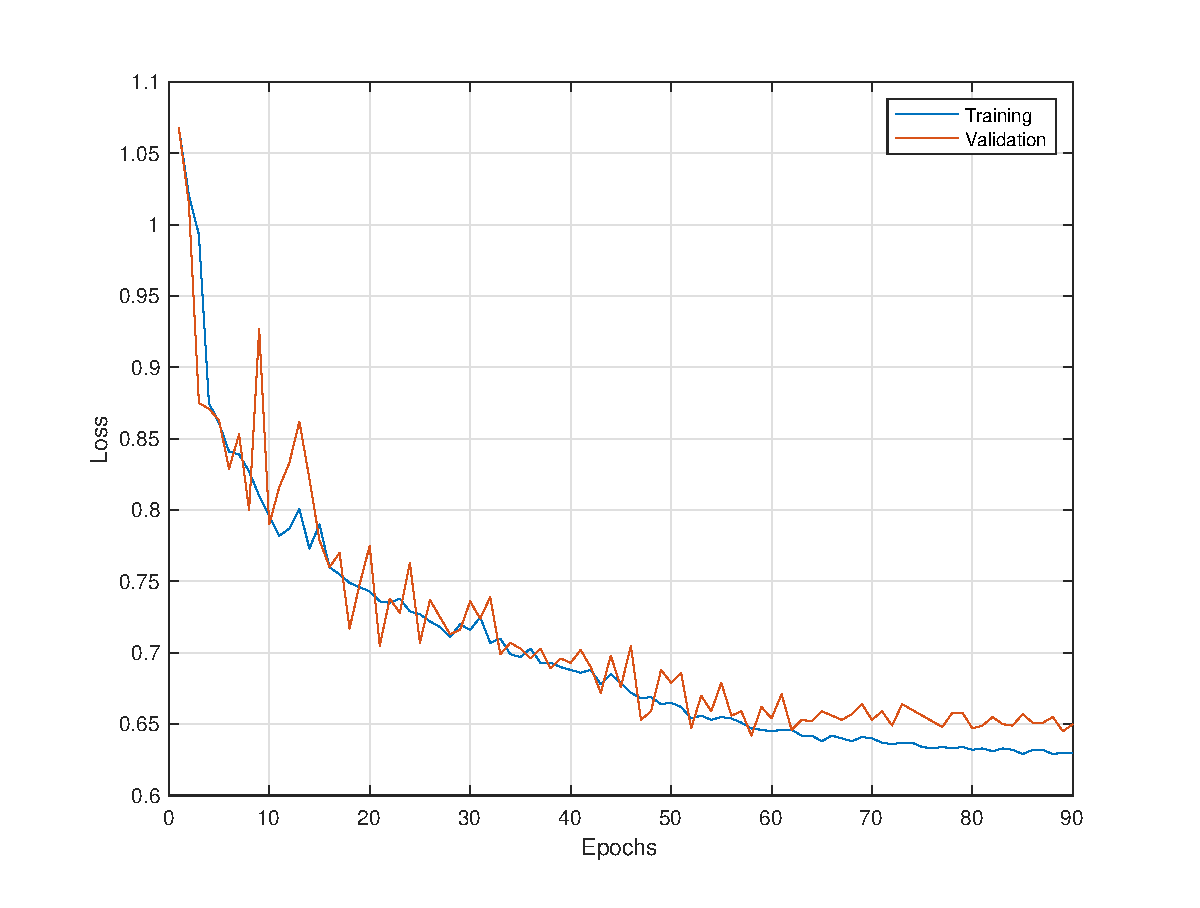
\includegraphics[width=0.7\textwidth]{./fig/photos/loss.eps}
  \caption{Loss during the training process.}
  \label{fig:loss}
\end{figure}


\section{Navigation algorithm}

Two different approaches were tested in this thesis. The first is angular and forward velocity generation, the second is path generation in combination with a collision free pathfinding algorithm. 

\subsection{Velocity generation}

Generating velocities is the most intuitive way to utilise the neural network for trail following. In this case, input to the vehicle are only two values: angular velocity for heading correction and forward velocity for moving along the path when it is safe according to the neural network outputs. Angular velocity $\omega$ can be calculated using a simple formula

\begin{equation}
	\omega = (\textrm{p}(\textrm{RIGHT}) - \textrm{p}(\textrm{LEFT}))\cdot\omega_{max}\,,
\end{equation}
where $\textrm{p}(\textrm{RIGHT})$ is the probability of the current direction being "right", $\textrm{p}(\textrm{LEFT})$ is the probability of the current direction being "left", $\omega_{max}$ is the maximum desired angular velocity. Forward speed $v_x$ is calculated according to a formula:

\begin{equation}
	v_x = \textrm{p}(\textrm{STRAIGHT})\cdot v_{max}\,,
\end{equation}
where $\textrm{p}(\textrm{STRAIGHT})$ is the probability of the current direction being "straight" and $v_{max}$ is the maximum desired longtitudinal velocity.


\subsection{Path generation}

\acs{MRS} \acs{ROS}-based system allows to control a \acs{UAV} using paths. They are represented as a sequence of geometric poses, which a vehicle should take. The implemented neural network does not allow to predict a future direction of travel and gives an output only for the current position. Therefore, it is possible to predict only one point of the path on every image pass through the neural network. This point can be immediately sent to a path planner. Such approach has a big advantage: the algorithm can be run simultaneously with obstacle avoidance and other features. Path planner can then decide whether suggested direction is safe or other maneuver must be taken to evade a collision. A point is given to the system in a format of \texttt{Reference} \acs{MRS} message. It consists of a \texttt{float64} value "heading" and a \texttt{Point} message "position", formed by three \texttt{float64} values for the position in x, y and z axes. Therefore, each point is described by 4 \texttt{float} values. These points can be represented relative to the \acs{UAV} current position with tilt-correction (xy plane is always parallel to the ground and z is always perpendicular). 

Heading $\alpha$ for the path point is calculated according to the formula:

\begin{equation}
	\alpha = (\textrm{p}(\textrm{RIGHT}) - \textrm{p}(\textrm{LEFT}))\cdot \alpha_{max}\,,
\end{equation}
where $\alpha_{max}$ is the maximum desired increment in radians. Step in x-axis $r_x$ relative to the current position is calculated as

\begin{equation}
	r_x = \textrm{p}(\textrm{STRAIGHT})\cdot \textrm{cos}(\alpha)\cdot r_{max}\,,
\end{equation}
where $r_{max}$ is a maximum desired step length. Step in y-axis $r_y$ is calculated as
\begin{equation}
	r_y = \textrm{p}(\textrm{STRAIGHT})\cdot \textrm{sin}(\alpha)\cdot r_{max}\,.
\end{equation}
Altitude is considered to remain constant so for each point it is set to $(1.8\,\textrm{m} - actual\_height)$ above the ground. Similar altitude was used in the dataset. Parameters $\alpha_{max}$, $r_{max}$ can be calibrated for better performance.

Such policy was used during the experiments because the ability to combine the algorithm with a path planner is a priority.

\subsection{Filtering of the neural network output}

The implemented neural network produces results online, at 30\,Hz. During operation, a lens flare or other short-term disturbance can occur. It leads to rapid changes in the prediction and combined with the path generation creates wrong, potentially unsafe points in a trajectory. Therefore, the output must be filtered. To get rid of high frequency changes, a low-pass filter is used. In this thesis, a simple yet effective low pass filter was employed: a moving average filter. For frame number $n$, it also remembers $k-1$ previous predictions and outputs average of these $k$ predictions. Value $k=15$ showed good results during tests and thus was used in this work. Its formula is
\begin{equation}
	y_n = u_n + u_{n-1} + u_{n-2} + ... + u_{n-k+1}\,,
\end{equation}
where $y_i$ is the output of the filter for the frame number $i$, $u_i$ is the raw output from the neural network for the frame number $i$.


\chapter{Simulation}

%TODO: Describe how to install and run the simulation.

%TODO: Describe how do I get data from the drone and then send commands.

\section{Software}

For simulation of such complex application, a dedicated software is needed. The main tool that was used for simulation and further usage on a real robot is the Robot Operating System (\acs{ROS}). It is a framework for robotic applications which offers abstraction from hardware, and even contains already implemented functions for communication between vehicles, sensors, cameras and other used hardware, both real and virtual. 
The communication is performed using high-level messages. For every hardware unit a node is created. These nodes can subscribe (receive information) or publish to some topic. A topic represents a virtual pipe, through which the information is transferred. For example, there is a program running on a robot PC. Program is subscribed to the topic \texttt{"/image"}, where the image is obtained from the node \texttt{"/camera"} and receives the image from it. Then, it processes the image, makes some decision after it and commands the speed using the \texttt{"/speed"} topic of the node \texttt{"/drone"}. Usually there are topics also for trajectory, odometry and other features \cite{quigley2009ros}.

Another tool used for simulation is Gazebo. It offers real-time graphical visualisation of the ongoing experiment. Realistic scenarios can be created in this simulator, its engine allows for shaders, different lighting conditions, and even physics simulation. Therefore, a virtual model of the use-case scene and conditions is usually designed, including the vehicle itself. Such model makes it possible to conveniently test the designed software before proceeding to real-world experiments as the cost of a mistake in the real world can be high. 

\section{Simulation setup}

For trail following simulation I decided to use the \acs{MRS} pre-configured setup for one-vehicle simulation (available at \url{https://github.com/ctu-mrs/simulation}). In my case, the system runs inside a singularity container. Default simulation does not include the onboard camera. Thus the front-facing camera was added to the robot model. "Baylands" world was selected for simulation, because it has a section of forest path in it. Overview of this world is on \reffig{fig:baylands}.

The code must be modified to be run in simulation. Only needed change is the topic, from which the images are received.

\begin{figure}[!h]

  \centering
  \includegraphics[width=0.75\textwidth]{./fig/photos/baylands.jpg}
  \caption{"Baylands" world. Image from \url{docs.px4.io}.}
  \label{fig:baylands}
\end{figure}


\section{Simulation results}

During the experiment in simulation, performance of the implemented algorithm was tested in close to real-world conditions. The \acs{MAV} successfully managed to follow the trail without getting lost (\reffig{fig:sim}). There were some oscillations during the heading correction, but these can be removed by using more complex heading regulation and fine tuning. The overall performance is good and the proposed methods for navigation along the path worked as expected. Vehicle stayed on the trail for as long as the simulation was going, without fails. However, the used map is relatively simple and has no obstacles or confusing factors. It was used to check the basic performance. Further and more detailed testing is conducted in real-world conditions, described in \refsec{rwexperiment}.


\begin{figure}[!h]

  \centering
  \subfloat[The neural network predicts that the \acs{MAV} is most likely pointed right relative to the path, when it is actually pointed right. Vehicle turns left.] {
    \includegraphics[width=0.75\textwidth]{./fig/photos/sim_right.png}
    \label{fig:sim_right}
  }

  \centering	
  

  \subfloat[Prediction "straight" is most likely, the \acs{MAV} is pointed straight. Vehicle moves forward.] {
    \includegraphics[width=0.75\textwidth]{./fig/photos/sim_straight.png}
    \label{fig:sim_straight}
  }

  \caption{Example images from the simulation.}
  \label{fig:sim}
\end{figure}







\chapter{Experiment}

\section{Neural network performance test}

For evaluation of the neural network performance in real-world forest conditions a preliminary experiment was conducted. The on-board computer and the camera were powered from  the battery and manually moved through the forest. Data was outputed in real-time to a laptop and the prediction correctness was evaluated (\reffig{fig:test_nn}).


\begin{figure}[!h]
  \begin{minipage}{.5\linewidth}
  \centering
  \subfloat[Camera pointed straight.] {
    \includegraphics[width=0.9\textwidth]{./fig/photos/nn_1_1.jpg}
    \label{fig:nn_1_1}
  }
  \end{minipage}
  \begin{minipage}{.5\linewidth}
  \centering	
  

  \subfloat[Prediction: "straight" is most likely.] {
    \includegraphics[width=0.9\textwidth]{./fig/photos/nn_2_1.jpg}
    \label{fig:nn_2_1}
  }
  \end{minipage}
  
  
  \begin{minipage}{.5\linewidth}
  \centering
  \subfloat[Camera is pointed left.] {
    \includegraphics[width=0.9\textwidth]{./fig/photos/nn_1_2.jpg}
    \label{fig:nn_1_2}
  }
  \end{minipage}
  \begin{minipage}{.5\linewidth}
  \centering	
  

  \subfloat[Prediction: "left" is most likely.] {
    \includegraphics[width=0.9\textwidth]{./fig/photos/nn_2_2.jpg}
    \label{fig:nn_2_2}
  }
  \end{minipage}
  
  \begin{minipage}{.5\linewidth}
  \centering
  \subfloat[Camera is pointed right.] {
    \includegraphics[width=0.9\textwidth]{./fig/photos/nn_1_3.jpg}
    \label{fig:nn_1_3}
  }
  \end{minipage}
  \begin{minipage}{.5\linewidth}
  \centering	
  

  \subfloat[Prediction: "right" is most likely.] {
    \includegraphics[width=0.9\textwidth]{./fig/photos/nn_2_3.jpg}
    \label{fig:nn_2_3}
  }
  \end{minipage}
  
  
  \caption{Neural network performance in the preliminary experiment.}
  \label{fig:test_nn}
\end{figure}

The testing showed good neural network performance. The accuracy of determining the "left" and "right" classes in tested situations was 100\%. There was once a situation though, where the neural network was outputting a small probability of "straight" class, when looking straight. Probabilities of "left" and "right" were the same, close to 50\%. But the issue was clearly dependent on the tilt angle of the camera, after tilting it a few degrees down, the problem was solved. A possible source of the issue could be not only the neural network fail-case, but also a lens flare.

\section{Complete tests on the vehicle}
\label{rwexperiment}

A real-world evaluation was conducted in a forest near the Czech town Temešvár. Together with the \acs{MRS} team, suitable forest trails were found, where the algorithm was then thoroughly tested. Trails are of different complexity (visually) and contain slight obstacles on the sides (\reffig{fig:trails}). 

\begin{figure}[!h]

  \centering
  \subfloat[Trail 1.] {
    \includegraphics[width=0.72\textwidth]{./fig/photos/path_1_op.png}
    \label{fig:path_1}
  }

  \centering	
  

  \subfloat[Trail 2.] {
    \includegraphics[width=0.72\textwidth]{./fig/photos/path_2_op.png}
    \label{fig:path_2}
  }

  \centering
  \subfloat[Trail 3.] {
    \includegraphics[width=0.72\textwidth]{./fig/photos/path_3_op.png}
    \label{fig:path_3}
  }
  \caption{The three trails used for testing in the real-world experiments.}
  \label{fig:trails}
\end{figure}

The first trail (\reffig{fig:path_1}) is a 2.3\,m wide partly dirty asphalt road with turns, surrounded by trees and bushes. Due to the limited \acs{FOV} of the camera and a relatively wide trail, when the vehicle was in the centre of the road, it saw only a grey dull pattern with no features and because of that outputed 100\% probability of "straight" class even when not pointed straight. But as soon as the \acs{UAV} got close to the road edge, the neural network recognised it and gave the command to turn in the opposite direction. Then, it started flying along the path and slowly got closer to the other side and the same situation happened. However, this "zig-zag" behaviour does not affect the performance too much. But in some situations, flying close to the road edge is dangerous and during this test, the path planner prevented the vehicle from executing several waypoints due to their proximity to an obstacle (\reffig{fig:avoid_1}). The problem can be solved by using a camera with a wider \acs{FOV}. The autonomously travelled distance on the first path was 130\,m (\reffig{fig:satellite_1}).

\begin{figure}[!h]

  \centering
  \subfloat[\acs{UAV} avoiding an obstacle.] {
    \includegraphics[width=0.7\textwidth]{./fig/photos/path_1_avoid.png}
    \label{fig:avoid_1}
  }

  \centering	
  

  \subfloat[Satellite image of the travelled path from Google Maps.] {
    \includegraphics[width=0.7\textwidth]{./fig/photos/path_1.png}
    \label{fig:satellite_1}
  }

  \caption{The first experiment.}
  \label{fig:first_trail_photos}
\end{figure}


The second trail (\reffig{fig:path_2}) is a 2-2.3\,m wide completely dirt road with one sharp turn and fences on sides. It was hard for the \acs{MAV} to stay on it. A lot of distracting features were present on the road and the trail itself was not well maintained. When analysing the images, it can be seen that the contrast between the trail and dry grass on the sides is very low. Probably, colour adjustments of the camera are required and also including such low-contrast images to the dataset would help. Also, there was a ditch on the road which looked like a trail for the \acs{MAV} (\reffig{fig:confused_2}). However, when the obstacle avoidance prevented it from flying into the bush, the real trail reappeared in the field of view and the vehicle managed to return on track. At the end, it got distracted again. Such trail was not followed with much success, but after the mentioned improvements, the results should be better. The total autonomously travelled distance on this path was 40\,m (\reffig{fig:satellite_2}).


\begin{figure}[!h]

  \centering
  \subfloat[\acs{MAV} got confused by a ditch, photo before recovery.] {
    \includegraphics[width=0.72\textwidth]{./fig/photos/path_2_confused.png}
    \label{fig:confused_2}
  }

  \centering	
  

  \subfloat[Satellite image of the travelled path from Google Maps.] {
    \includegraphics[width=0.72\textwidth]{./fig/photos/path_2.png}
    \label{fig:satellite_2}
  }

  \caption{The second experiment.}
  \label{fig:second_trail_photos}
\end{figure}

The third trail (\reffig{fig:path_3}) is a 2.8\,m wide gravel and dirt road with slight turns. Contrast between the road and sides on the gravel part is better than on previous trails. On the dirt part contrast gets much lower, distinction between the trail and sides is not as clear. But it has not confused the \acs{CNN}. Its performance was better than on other trails. The \acs{MAV} flew a long way through it. However, in the end it got confused by logs on the ground and the vehicle started "following" one of them (\reffig{fig:fail_log_3}). It may have happened due to the road and the sides being both covered in dirt and from the vehicle camera perspective they were not distinguishable. The total path flown autonomously was 160\,m on this trail (\reffig{fig:satellite_3}). Images from the \acs{MAV} including the prediction are presented on \reffig{fig:onboard}.

During the experiments, the vehicle was mapping the environment with the \acs{LiDAR}. These maps are presented on \reffig{fig:lidar}. Approximately every meter the position and the direction of the drone are visualised using a red arrow. The performance of the implemented algorithm can be seen from them. The obstacle avoidance did not change the heading, so all the heading corrections during the flight were made only by the trail following program. According to those images, the vehicle performed very good when flying through the first and the third trail. The arrows are pointed along the safe path.

\begin{table}[]
\centering
\begin{tabular}{|l|l|l|}
\hline
Experiment number & Travelled distance (m) & Flight time (minutes) \\ \hline
1                 & 130                    & 6:50                  \\ \hline
2                 & 40                     & 3:00                  \\ \hline
3                 & 160                    & 6:11                  \\ \hline
\end{tabular}
\caption{Experiment statistics.}
\end{table}

\begin{figure}[!h]

  \centering
  \subfloat[\acs{MAV} got confused by the log.] {
    \includegraphics[width=0.72\textwidth]{./fig/photos/path_3_fail_log.png}
    \label{fig:fail_log_3}
  }

  \centering	
  

  \subfloat[Satellite image of the travelled path from Google Maps.] {
    \includegraphics[width=0.72\textwidth]{./fig/photos/path_3.png}
    \label{fig:satellite_3}
  }

  \caption{The third experiment.}
  \label{fig:third_trail_photos}
\end{figure}


\begin{figure}[!h]
  \begin{minipage}{.5\linewidth}
  \centering
  \subfloat[The first trail.] {
    \includegraphics[width=0.85\textwidth]{./fig/photos/path1_lidar.png}
    \label{fig:lidar1}
  }
  \end{minipage}
  \begin{minipage}{.5\linewidth}
  \centering	
  \subfloat[The second trail.] {
    \includegraphics[width=0.85\textwidth]{./fig/photos/path2_lidar.png}
    \label{fig:lidar2}
  }
  \end{minipage}
  
  \centering	
  \subfloat[The third trail.] {
    \includegraphics[width=0.4\textwidth]{./fig/photos/path3_lidar1.png}
    \label{fig:lidar3}
  }

  \caption{Maps of the environment, obtained using \acs{LiDAR}.}
  \label{fig:lidar}
\end{figure}
% Onboard
\begin{figure}[!h]
  \begin{minipage}{.5\linewidth}
  \centering
  \includegraphics[width=0.85\textwidth]{./fig/photos/path3_camera.png}
  
  \end{minipage}
  \begin{minipage}{.5\linewidth}
  \centering	
  \includegraphics[width=0.85\textwidth]{./fig/photos/path3_camera2.png}
  
  \end{minipage}
  \caption{Onboard images and classification results.}
  \label{fig:onboard}
\end{figure}





\chapter{Conclusion}

%TODO: \include{csquotes}, potom \enquote{v uvozovkach}

In this thesis, a 3-class classification convolutional neural network was implemented to solve the trail following problem utilising a purely visual approach. Using only an RGB camera is a cheap solution and no other hardware than an onboard PC with a camera is required to run the program. Also, the neural network is supplemented by an algorithm, which generates path points according to the prediction. The program is able to run in the Gazebo simulator and in real-world conditions online and was tested in both virtual and real environments.

During the training process, the neural network showed up to 90\% accuracy on validation. However, the dataset that was employed for training, was acquired by other cameras than those used in this thesis. During the experiments, the vehicle was able to fly long distances on curvy trails (up to 160\,m) but got stuck when the trail was not contrast enough or distracting factors appeared in the image. This problem can be caused by a different \acs{FOV} of the used camera, colour rendering, image sensor quality and even season. Therefore, the results can be improved by creating a new larger dataset with conditions close to the expected and training the network on it. Also, increasing the field of view could help, because more features can be captured by the camera.

Another possible improvement can be the usage of a segmentation neural network, as it allows to predict also the shape of the future trajectory. However, it may be challenging to distinguish the road from the sides during segmentation, and requires a big manually labeled dataset. Therefore, in this thesis only the classification approach was taken.

The implemented algorithm is a good baseline and an addition for more complex navigation solutions in forest conditions. It was demonstrated during experiments, when \acs{LiDAR}-based obstacle avoidance and path planning run alongside with the trail-following neural network. It prevented the \acs{UAV} from flying too close to dangerous obstacles like trees or bushes.

The \acs{MAV} flew autonomously up to 160\,m in a challenging forest environment using the proposed approach and the implemented program.


%% |                         References                         |
%% --------------------------------------------------------------

\chapter{References}

\printbibliography[heading=none,title={}]

%% --------------------------------------------------------------
%% |                         Appendices                         |
%% --------------------------------------------------------------

%\appendix
%\renewcommand\chaptername{Appendix}

%\renewcommand{\thechapter}{A}
%\renewcommand\chaptername{Appendix A}

%\chapter{Appendix A}

\end{document}
